El diseño atómico es una metodología compuesta por cinco etapas distintas que trabajan juntas para crear sistemas de diseño de interfaz de una manera más deliberada y jerárquica. Las cinco etapas del diseño atómico son:
\vspace{0.8cm}

\begin{enumerate}
  \item Átomos
  \item Moléculas
  \item Organismos
  \item Plantillas
  \item Páginas
\end{enumerate}
\vspace{0.8cm}

El diseño atómico no es un proceso lineal, sino un modelo mental que nos ayuda a pensar en nuestras interfaces de usuario como un todo cohesivo y una colección de partes al mismo tiempo. Cada una de las cinco etapas juega un papel clave en la jerarquía de nuestros sistemas de diseño de interfaz \cite{frost}.
\vspace{0.8cm}


\begin{figure}[H]
  \centering
  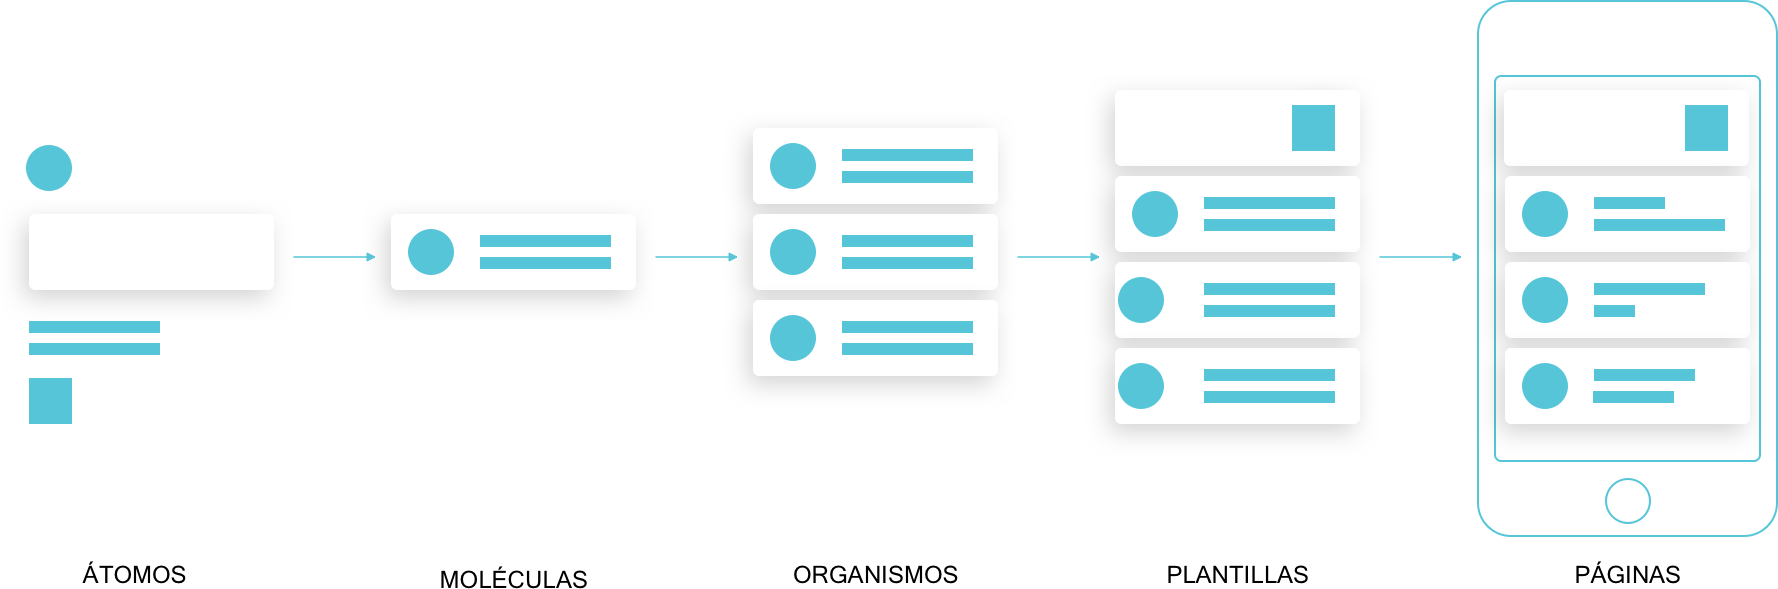
\includegraphics[width=1\textwidth]{atomic}
  \caption{Metodología de diseño atómico.}
\end{figure}